\chapter{Statistica descrittiva}
\label{chapter:descriptive_stats}


Nel 1907 Francis Galton, cugino di Charles Darwin, matematico e statistico autodidatta, geografo, esploratore, teorico della dattiloscopia (ovvero, dell'uso delle impronte digitali a fini identificativi) e dell'eugenetica, scrisse una lettera alla rivista scientifica Nature sulla sua visita alla \emph{Fat Stock and Poultry Exhibition} di Plymouth. 
Lì vide alcuni membri del pubblico partecipare ad un gioco il cui scopo era quello di  indovinare il peso della carcassa di un grande bue che era appena stato scuoiato.
Galton si procurò i 787 dei biglietti che erano stati compilati dal pubblico e considerò il valore medio di 547 kg come la \enquote{scelta democratica} dei partecipanti, in quanto \enquote{ogni altra stima era stata giudicata troppo alta o troppo bassa dalla maggioranza dei votanti}.
Il punto interessante è che il peso corretto di 543 kg si dimostrò essere molto simile alla \enquote{scelta democratica} basata sulle stime dei 787 partecipanti. 
Galton intitolò la sua lettera a Nature \emph{Vox Populi} (voce del popolo), ma questo processo decisionale è ora meglio conosciuto come la \enquote{saggezza delle folle} (\emph{wisdom of crowds}).
Possiamo dire che, nel suo articolo del 1907, Galton effettuò quello che ora chiamiamo un riepilogo dei dati, ovvero calcolò un indice sintetico a partire da un insieme di dati.
In questo capitolo esamineremo le tecniche che sono state sviluppate nel secolo successivo per riassumere le grandi masse di dati con cui sempre più spesso ci dobbiamo confrontare.
Vedremo come calcolare e interpretare gli indici di posizione e di dispersione, discuteremo le distribuzioni di frequenze e le relazioni tra variabili.
Vedremo inoltre quali sono le tecniche di visualizzazione che ci consentono di rappresentare questi sommari dei dati mediante dei grafici. 
Ma prima di entrare nei dettagli, prendiamoci un momento per capire perché abbiamo bisogno della statistica descrittiva.


\section{Perché riassumere i dati?}

Quando riassumiamo i dati, necessariamente buttiamo via delle informazioni. 
Ma è una buona idea procedere in questo modo? 
Non sarebbe meglio conservare le informazioni specifiche di ciascun soggetto che partecipa ad un esperimento psicologico, al di là di ciò che viene trasmesso dagli indici riassuntivi della statistica descrittiva? 
Che dire delle informazioni che descrivono come sono stati raccolti i dati, come l'ora del giorno o l'umore del partecipante? 
Tutte queste informazioni vengono perdute quando riassumiamo i dati.
La risposta alla domanda che ci siamo posti è che, in generale, non è una buona idea conservare tutti i dettagli di ciò che sappiamo.
È molto più utile riassumere le informazioni perché la semplificazione risultante consente i processi di generalizzazione.

In un contesto letterario, l'importanza della generalizzazione è stata sottolineata da Jorge Luis Borges nel suo racconto \enquote{Funes o della memoria}, che descrive un individuo che perde la capacità di dimenticare. 
Borges si concentra sulla relazione tra generalizzazione e pensiero: \enquote{Pensare è dimenticare una differenza, generalizzare, astrarre. 
Nel mondo troppo pieno di Funes, c'erano solo dettagli}.
Come possiamo ben capire, la vita di Funes non è facile.
Se facciamo riferimento alla psicologia possiamo dire che gli psicologi hanno studiato a lungo l'utilità della generalizzazione per il pensiero. 
Un esempio è fornito dal fenomeno della formazione dei concetti e lo psicologo che viene in mente a questo proposito è sicuramente Eleanor Rosch, la quale ha studiato i principi di base della categorizzazione.
I concetti ci forniscono uno strumento potente per organizzare le conoscenze.
Noi siamo in grado di riconoscere facilmente i diversi esemplare di un concetto -- per esempio,  \enquote{gli uccelli} -- anche se i singoli esemplari che fanno parte di una categoria sono molto diversi tra loro (l'aquila, la gallina, il pettirosso). 
L'uso dei concetti, cioè la generalizzazione, è utile perché ci consente di fare previsioni sulle proprietà dei singoli esemplari che appartengono ad una categoria, anche se non abbiamo mai avuto esperienza diretta con essi -- per esempio, possiamo fare la predizione che tutti gli uccelli possono volare e mangiare vermi, ma non possono guidare un'automobile o parlare in inglese. 
Queste previsioni non sono sempre corrette, ma sono utili. 

Le statistiche descrittive, in un certo senso, ci fornisco l'analogo dei \enquote{prototipi} che, secondo Eleanor Rosch, stanno alla base del processo psicologico di creazione dei concetti.
Un prototipo è l'esemplare più rappresentativo di una categoria.
In maniera simile, una statistica descrittiva come la media, ad esempio, potrebbe essere intesa come l'osservazione \enquote{tipica}.

La statistica descrittiva ci fornisce gli strumenti per riassumere i dati che abbiamo a disposizione in una forma visiva o numerica.
Le rappresentazioni grafiche più usate della statistica descrittiva sono gli istogrammi, i diagrammi a dispersione o i box-plot, e gli indici sintetici più comuni sono la media, la mediana, la varianza e la deviazione standard.


\section{Distribuzioni di frequenze}
\label{sec:distr_freq}

Per introdurre i principali strumenti della statistica descrittiva considereremo qui i dati raccolti da \citet{zetsche_future_2019}. 
Questi autori hanno studiato le aspettative negative le quali sono state evidenziate come un meccanismo chiave nel mantenimento e nella reiterazione della depressione. 
\citet{zetsche_future_2019} hanno valutato le aspettative di individui depressi circa il loro umore futuro ed si sono chiesti se queste aspettative fossero accurate oppure distorte negativamente. 
In uno degli studi descritti viene esaminato un campione costituito da 30 soggetti con almeno un episodio depressivo maggiore e da 37 controlli sani. 
Gli autori hanno misurato il livello depressivo con il \emph{Beck Depression Inventory} (BDI-II).
Ma qual è la la gravità della depressione riportata dai soggetti nel campione esaminato da \citet{zetsche_future_2019}?
Dei 67 soggetti considerati, uno non ha completato il BDI-II e quindi rimaniamo con 66 valori del BDI-II.
I dati sono riportati nella tabella~\ref{tab:Zetsche2020} (per semplicità sono stati ordinati in ordine crescente). 
È chiaro che i dati grezzi sono di difficile lettura. 
Poniamoci dunque il problema di creare una rappresentazione sintetica e comprensibile di questo insieme di valori.

\begin{table}[h!]
\scriptsize
\caption{Valori del BDI-II riportati da \citet{zetsche_future_2019} nel campione clinico e di controllo.}
\label{tab:Zetsche2020}
\centering
\begin{tabular}{ccccccccccccccccc}
 \toprule
0 & 0 & 0 & 0 & 0 & 0 & 0 & 0 & 0 & 0 & 0 & 0 & 0 & 0 & 0 & 0 & 0 \\ 
1 & 1 & 1 & 1 & 1 & 1 & 1 & 1 & 2 & 2 & 2 & 2 & 3 & 3 & 3 & 5 & 7 \\
9 & 12 & 19 & 22 & 22 & 24 & 25 & 25 & 26 & 26 & 26 & 27 & 27 & 28 & 28 & 30 & 30 \\ 
30 & 31 & 31 & 33 & 33 & 34 & 35 & 35 & 35 & 36 & 39 & 41 & 43 & 43 & 44 & & \\
 \bottomrule
\end{tabular}
\end{table}

Uno dei modi che ci consentono di effettuare una sintesi dei dati è quello di generare una \emph{distribuzione di frequenze}.
\begin{defn}
Una distribuzione di frequenze è un riepilogo del conteggio della frequenza con cui le modalità osservate in un insieme di dati si verificano in un intervallo di valori. 
\end{defn}
Per creare una distribuzione di frequenze possiamo procedere effettuando una partizione delle modalità della variabile di interesse in $m$ classi (denotate con $\Delta_i$) tra loro disgiunte.  
In tale partizione, la classe $i$-esima coincide con un intervallo di valori aperto a destra $[a_i, b_i)$ o aperto a sinistra $(a_i, b_i]$\footnote{
Un intervallo aperto non include i suoi estremi ed è indicato con le parentesi tonde. 
Ad esempio, (0,1) significa maggiore di 0 e minore di 1. 
Un intervallo chiuso è un intervallo che include i suoi estremi ed è indicato con le parentesi quadre.
Ci possono essere intervalli aperti, ``$(a, b)$'', intervalli chiusi, ``$[a, b]$'', intervalli aperti a sinistra, ``$(a, b]$'', e intervalli aperti a destra, ``$[a, b)$''.
}.
Ad ogni classe $\Delta_i$ avente $a_i$ e $b_i$ come limite inferiore e superiore  associamo l'ampiezza $b_i - a_i$ (non necessariamente uguale per ogni classe) e il valore centrale $\bar{x}_i$. 
La scelta delle classi è arbitraria, ma è buona norma non definire classi con un numero troppo piccolo (< 5) di osservazioni. 
Poiché ogni elemento dell'insieme $\{x_i\}_{i=1}^n$ appartiene ad una ed una sola classe $\Delta_i$, possiamo calcolare le quantità elencate di seguito.
\begin{description}
\item[La frequenza assoluta] $n_i$ di ciascuna classe, ovvero il numero di osservazioni che ricadono nella classe $\Delta_i$. Proprietà: $n_1 + n_2 + \dots + n_m = n$.
\item[La frequenza relativa] $f_i = n_i/n$ di ciascuna classe. 
Proprietà: $f_1+f_2+\dots+f_m =1$.
\item[La frequenza cumulata] $N_i$, ovvero il numero totale delle osservazioni che ricadono nelle classi fino alla $i$-esima compresa:
$N_i = \sum_{i=1}^m n_i.$
\item[La frequenza cumulata relativa] $F_i$, ovvero $F_i = 
%f_1+f_2+\dots+f_m = \frac{N_i}{n}= 
%\frac{1}{n} 
\sum_{i=1}^m f_i.$
\end{description}

Calcoliamo ora le distribuzioni di frequenze frequenze assolute e relative per i valori del BDI-II di \citet{zetsche_future_2019}. 
Per costruire una distribuzione di frequenza è innanzitutto necessario scegliere gli intervalli delle classi.
Facendo riferimento ai cut-off usati per l'interpretazione del BDI-II, definiamo i seguenti intervalli aperti a destra:
depressione minima: [0, 13.5),
depressione lieve: [13.5, 19.5),
depressione moderata: [19.5, 28.5),
depressione severa: [28.5, 63).

La distribuzione di frequenza dei dati della tabella~\ref{tab:Zetsche2020} è riportata nella tabella~\ref{tab:Zetsche2020_freq}.
Questa tabella ci aiuta a capire meglio cosa sta succedendo.
Se consideriamo le frequenze relative, ad esempio, possiamo notare che ci sono due valori maggiormente ricorrenti nella distribuzione di frequenze e tali valori corrispondono alle due classi più estreme.
Questo ha senso nel caso presente, in quanto il campione esaminato da \citet{zetsche_future_2019} includeva due gruppi di soggetti: soggetti sani (con valori BDI-II bassi) e soggetti depressi (con valori BDI-II alti).
In una distribuzione di frequenze tali valori tipici vanno sotto il nome di \emph{mode} della distribuzione.

\begin{table}
\caption{Distribuzioni di frequenza per i dati della tabella~\ref{tab:Zetsche2020}.}
\centering
\begin{tabular}{ccccc}
\hline
Limiti delle classi & Freq. ass. & Freq. rel. & Freq. ass. cum. & Freq. rel. cum.\\
\hline
$[0, 13.5)$  & 36 & 36/66 &  36 &  36/66\\
$[13.5, 19.5)$ & 1  & 1/66  &  37 &  37/66\\
$[19.5, 28.5)$ & 12 & 12/66 &  49 &  49/66\\
$[28.5, 63)$ & 17 & 17/66 &  66 &  66/66\\
\hline
\end{tabular}
\label{tab:Zetsche2020_freq}
\end{table}


\subsection{Istogramma}

I dati che sono stati sintetizzati in una distribuzione di frequenze possono essere rappresentati graficamente in un istogramma. 
Poniamoci dunque il problema di costruire un istogramma per i dati del BDI-II.

Un istogramma si costruisce riportando sulle ascisse i limiti delle classi $\Delta_i$ e sulle ordinate i valori della funzione costante a tratti
\begin{equation}
\varphi_n(x)= \frac{f_i}{b_i-a_i}, \quad x\in \Delta_i,\, i=1, \dots, m
\end{equation}
che misura la \emph{densità della frequenza relativa} della variabile $X$ nella classe $\Delta_i$, ovvero il rapporto fra la frequenza relativa $f_i$ e l'ampiezza ($b_i - a_i$) della classe. 
In questo modo il rettangolo dell'istogramma associato alla classe $\Delta_i$ avrà un'area proporzionale alla frequenza relativa $f_i$. 
Si noti che l'area totale dell'istogramma delle frequenze relative è data della somma delle aree dei singoli rettangoli e quindi vale 1.0. 

Con i quattro intervalli individuati dai cut-off del BDI-II otteniamo la rappresentazione riportata nel pannello di sinistra della figura~\ref{fig:Zetsche_hist_plot}. 
Nel caso della prima barra dell'istogramma a sinistra, l'ampiezza dell'intervallo è pari a 13.5 e l'area della barra (ovvero, la frequenza relativa) è uguale a 36/66. 
Dunque l'altezza della barra è uguale a $(36 / 66) / 13.5 = 0.040$.
Lo stesso procedimento si applica per il calcolo dell'altezza degli altri rettangoli.

\begin{figure}
 \centering
 \includegraphics[width=\textwidth]{Zetsche_hist_plot.pdf}
 \caption{Istogramma per i dati della tabella~\ref{tab:Zetsche2020}. 
 Gli gli intervalli delle classi hanno ampiezze diverse nel pannello di sinistra e ampiezze uguali nel pannello di destra.}
\label{fig:Zetsche_hist_plot}
\end{figure}

Anche se nel caso presente è sensato usare ampiezze diverse per gli intervalli delle classi, in generale gli istogrammi si costruiscono utilizzando intervalli riportati sulle ascisse con un'ampiezza uguale.
Questo è il caso dell'istogramma riportato a destra della figura~\ref{fig:Zetsche_hist_plot} e generato a partire dagli stessi dati. 


\subsection{Funzione di densità empirica}

Il confronto tra i due pannelli della figura~\ref{fig:Zetsche_hist_plot} rende chiaro un limite degli istogrammi. 
È infatti ovvio che il profilo dell'istogramma è arbitrario: a seconda del numero e dei limiti delle classi che vengono scelte, cambiano sia il numero che la forma delle barre dell'istogramma.
Questo rende difficile fornire un'interpretazione alle informazioni fornite da un istogramma.

Il problema precedente può essere alleviato utilizzando una rappresentazione alternativa della distribuzione di frequenza, ovvero la stima della densità della frequenza dei dati (detta anche stima kernel di densità). 
Un modo semplice per pensare a tale rappresentazione, che in inglese va sotto il nome di \emph{density plot}, è quello di immaginare un grande campione di dati, in modo che diventi possibile definire un enorme numero di classi di equivalenza di ampiezza molto piccola, le quali non risultino vuote. 
In tali circostanze, la funzione di densità empirica non è altro che il profilo \enquote{lisciato} dell’istogramma. 
La stessa idea si applica anche quando il campione è più piccolo. 
Nel caso dei dati del BDI-II otteniamo la reppresentazione fornita dalla figura~\ref{fig:Zetsche_dens_plot}. 

Che interpretazione possiamo attribuire alla figura~\ref{fig:Zetsche_dens_plot}? 
La interpretiamo come abbiamo fatto in precedenza con gli istogrammi: l'area sottesa al grafico della funzione di densità empirica in un certo intervallo rappresenta la proporzione dei casi della distribuzione che hanno valori compresi nell'intervallo considerato.

\begin{figure}%[h!]
 \centering
 \includegraphics[width=\textwidth]{Zetsche_dens_plot.pdf}
 \caption{Istogramma per i dati della tabella~\ref{tab:Zetsche2020} con sovrapposta la funzione di densità empirica e, a destra, solo la funzione di densità empirica.}
 \label{fig:Zetsche_dens_plot}
 \end{figure}


\subsection{Forma di una distribuzione}

In generale, la forma di una distribuzione descrive come i dati si distribuiscono intorno ai valori centrali.
Distinguiamo tra distribuzioni simmetriche e asimmetriche, e tra distribuzioni unimodali o multimodali.
Un'illustrazione grafica è fornita nella figura~\ref{fig:simm_asim_bimod_distr}.
Nel pannello 1 la distribuzione è unimodadle con asimmetria negativa;
nel pannello 2 la distribuzione è unimodadle con asimmetria positiva;
nel pannello 3 la distribuzione è simmetrica e unimodale;
nel pannello 4 la distribuzione è bimodale.
Se consideriamo nuovamente la figura~\ref{fig:Zetsche_dens_plot} che riporta la densità della frequenza dei dati di \citet{zetsche_future_2019} è facile concludere che la distribuzione dei valori del BDI-II è bimodale.

\begin{figure}%[h!]
\centering
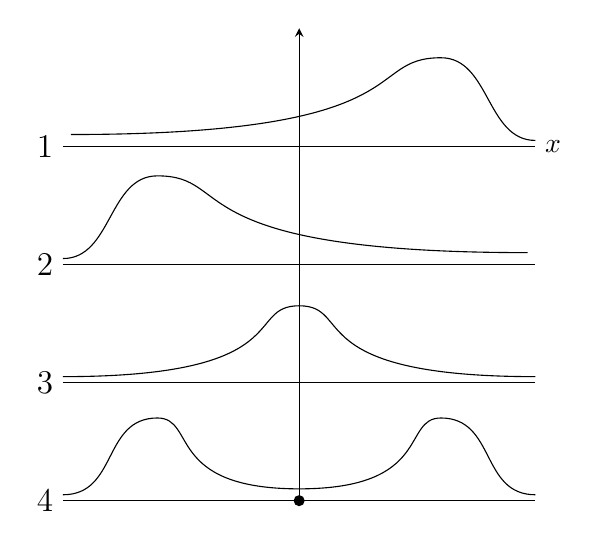
\begin{tikzpicture}[y=1.5cm]
\foreach [count=\i] \y in {4,3,2,1}
   \draw (0,\y) node [left,font=\large]{$\i$} -- (6,\y );
\node [right] at (6,4) {$x$};

\draw (0,3.05) to[out=0,in=180] ++(1.2,0.7) .. controls +(1,0) and  +(-4.5,0) .. ++(4.7,-0.65);
\draw (0,2.05) .. controls +(3,0) and  +(-0.7,0) .. (3,2.65) .. controls +(0.7,0) and +(-3,0) .. (6,2.05);
\draw (0,1.05) .. controls +(.7,0) and +(-.7,0)  .. (1.2,1.7) 
               .. controls +(0.5,0) and  +(-1.7,0) .. (3,1.1)
               .. controls +(1.7,0) and  +(-0.5,0) .. (4.8,1.7)
               .. controls +(0.7,0) and  +(-.7,0) .. (6,1.05);
\draw (6,4.05) to[out=180,in=0] ++(-1.2,0.7) .. controls +(-1,0) and  +(4.5,0) .. ++(-4.7,-0.65);

\fill (3,1) circle[radius=2pt];
\draw [-stealth] (3,1) -- (3,5);
\end{tikzpicture}
\caption{1: Asimmetria negativa. 2: Asimmetria positiva. 3: Distribuzione unimodale. 4: Distribuzione bimodale.}
\label{fig:simm_asim_bimod_distr}
\end{figure}


\section{Indici di posizione}

\subsection{Quantili}

La descrizione della distribuzione dei valori BDI-II di \citet{zetsche_future_2019} può essere facilitata dalla determinazione di alcuni valori caratteristici che sintetizzano le informazioni contenute nella distribuzione di frequenze. 
Si dicono \emph{quantili} (o \emph{frattili}) quei valori caratteristici che hanno le seguenti proprietà. 
I \emph{quartili} sono quei valori che ripartiscono i dati $x_i$ in quattro parti ugualmente numerose (pari ciascuna al 25\% del totale).
Il primo quartile, $q_1$, lascia alla sua sinistra il 25\% del campione pensato come una fila ordinata (a destra quindi il 75\%). 
Il secondo quartile $q_2$ lascia a sinistra il 50\% del campione (a destra quindi il 50\%).
Esso viene anche chiamato \emph{mediana}.
Il terzo quartile lascia a sinistra il 75\% del campione (a destra quindi il 25\%).
Secondo lo stesso criterio, si dicono \emph{decili} i quantili di ordine $p$ multiplo di 0.10 e \emph{percentili} i quantili di ordine $p$ multiplo di 0.01. 

Come si calcolano i quantili? 
Consideriamo la definizione di quantile \emph{non interpolato} di ordine $p$ $(0 < p < 1)$.
Si procede innanzitutto ordinando i dati in ordine crescente, $\{x_1, x_2, \dots, x_n\}$.
Ci sono poi due possibilità.
Se il valore $np$ non è intero, sia $k$ l'intero tale che $k < np < k + 1$ -- ovvero, la parte intera di $np$. 
Allora 
$
q_p = x_{k+1}.
$
Se $np = k$ con $k$ intero, allora
$
q_p = \frac{1}{2}(x_{k} + x_{k+1}).
$
Se vogliamo calcolare il primo quartile $q_1$, ad esempio, utilizziamo $p = 0.25$. 
Dovendo calcolare gli altri quantili basta sostituire a $p$ il valore appropriato\footnote{
Si noti che solitamente i software restituiscono un valore \emph{interpolato} di $p$-esimo quantile $q_p$ $(0 < p < 1)$, il quale viene calcolato mediante specifiche procedure.
Il risultato fornito dai software, dunque, non sarà identico a quello trovato utilizzando la definizione non interpolata di quantile che abbiamo presentato sopra.
Se, per qualche ragione, vogliamo conoscere l'algoritmo usato per la determinazione dei quantili interpolati, dobbiamo leggere la documentazione del software.
}.

Facciamo un esempio numerico considerando soltanto i nove soggetti del campione clinico di \citet{zetsche_future_2019} che hanno riportato un unico episodio di depressione maggiore.
Per tali soggetti i valori ordinati del BDI-II (per semplicità li chiameremo $x$) sono i seguenti: 19, 26, 27, 28, 28, 33, 33, 41, 43.
Per il calcolo del secondo quartile (non interpolato), ovvero per il calcolo della mediana, dobbiamo considerare la quantità $np = 9 \cdot 0.5 = 4.5$, non intero.
Quindi, $q_1 = x_{4 + 1} = 27$.
Per il calcolo del quantile (non interpolato) di ordine $p = 2/3$ dobbiamo considerare la quantità $np = 9 \cdot 2/3 = 6$, intero.
Quindi, $q_{\frac{2}{3}} = \frac{1}{2} (x_{6} + x_{7}) = \frac{1}{2} (33 + 33) = 33$. 

Gli indici di posizione, tra le altre cose, hanno un ruolo importante, ovvero vengono utilizzati per creare una rappresentazione grafica di una distribuzione di valori che è molto popolare e può essere usata in alternativa ad un istogramma (in realtà vedremo poi come possa essere combinata con un istogramma).
Tale rappresentazione va sotto il nome di box-plot.


\subsection{Box-plot}

Il \emph{box-plot} (o diagramma a scatola) è uno strumento grafico utile al fine di ottenere informazioni circa la dispersione e l'eventuale simmetria o asimmetria di una distribuzione. 
Per costruire un box-plot si rappresenta sul piano cartesiano un rettangolo (cioè la ``scatola'') di altezza arbitraria la cui base corrisponde alla dist intanza interquartile (IQR = $q_{0.75} - q_{0.25}$). 
La linea interna alla scatola rappresenta la mediana $q_{0.5}$.
Si tracciano poi ai lati della scatola due segmenti di retta i cui estremi sono detti ``valore adiacente'' inferiore e superiore.
Il valore adiacente inferiore è il valore più piccolo tra le osservazioni che risulta maggiore o uguale al primo quartile meno la distanza corrispondente a 1.5 volte la distanza interquartile (si veda la figura~\ref{fig:boxplot}). 
Il valore adiacente superiore è il valore più grande tra le osservazioni che risulta minore o uguale a $Q_3+1.5$ IQR. 
I valori esterni ai valori adiacenti (chiamati \emph{valori anomali}) vengono rappresentati individualmente nel box-plot per meglio evidenziarne la presenza e la posizione.
\begin{figure}%[h!]
\centering
\begin{tikzpicture}[thick, scale=.83]
 \filldraw[fill=gray!20] (2,0) rectangle (5,1);% draw the box
 \draw (3,0) -- (3,1) node[above]{$\textsc{M}$};% draw the median
 \draw (5,0.5) -- (7,0.5);% draw right whisker
 \draw (2,0.5) -- (1,0.5);% draw left whisker
 \draw (7,0.39) -- (7,0.61);% draw vertical tab
 \draw (1,0.39) -- (1,0.61);% draw vertical tab
 \node[below] at (2,0) {$\textsc{$Q_1$}$};% label the hinge
 \node[below] at (5,0) {$\textsc{$Q_3$}$};% label the hinge
 \filldraw[ball color=gray!80,shading=ball] (4,0.5) circle
 (0.06cm) node[above]{$\bar{x}$};% the mean
 \draw[<->] (2.3, -0.3) -- (4.7, -0.3)
 node[pos=0.5,below]{$\textsc{IQR}$}; % mark the IQR fences
 \draw[<->] (2, -0.8) -- (0,-0.8)
 node[pos=0.5,below]{$\textsc{1.5*IQR}$}; % left inner fence
 \draw[<->] (2,-1.4) -- (-2, -1.4)
 node[pos=0.5,below]{$\textsc{3*IQR}$};% left outer fence
 \draw[<->] (5, -0.8) -- (8,-0.8)
 node[midway,below]{$\textsc{1.5*IQR}$}; % right inner fence
 \draw[<->] (5,-1.4) -- (10, -1.4)
 node[pos=0.5,below]{$\textsc{3*IQR}$};% right outer fence
 %
 \node[below] at (9,0.7) {$\textbf{*}$}; % mild outlier on the right
 \node[below] at (-2.4,0.7) {$o$}; % extreme outlier on the left
 \draw (-3,-2) -- (11,-2);
 \draw[snake=ticks,segment length=1cm] (-3,-2) -- (11.1,-2);
\end{tikzpicture}
\caption{Box-plot, laddove $M$ è la mediana, $\bar{x}$ è la media aritmetica e IQR è la distanza interquartile ($Q_3 - Q_1$).}
\label{fig:boxplot}
\end{figure}

Consideriamo ora un caso concreto nel quale viene utilizzato un box-plot.
Nel caso dei dati di \citet{zetsche_future_2019} riportati nella tabella~\ref{tab:Zetsche2020} ci chiediamo in che modo si differenziano le distribuzioni del BDI-II tra i due gruppi considerati, ovvero tra il gruppo dei pazienti e il gruppo di controllo.
La figura~\ref{fig:Zetsche_violin_plot} ci fornisce due rappresentazioni grafiche possibili che possono essere utilizzate per rispondere a questa domanda.  

\begin{figure}
\centering
\includegraphics[width=1.0\linewidth]{Zetsche_violin_plot.pdf}
\caption{Due versioni di un ``violin plot'' dei valori BDI-II per ciascun gruppo specificato nella tabella~\ref{tab:Zetsche2020}.}
\label{fig:Zetsche_violin_plot}
\end{figure}

Nella figura~\ref{fig:Zetsche_violin_plot} sinistra sono rappresentati i dati grezzi: questa è la pratica migliore quando il numero di osservazioni è piccolo. 
La linea curva che circonda (simmetricamente) le osservazioni è l'``istogramma lisciato'' che abbiamo descritto in precedenza.
Nella figura~\ref{fig:Zetsche_violin_plot} destra sono rappresentanti gli stessi dati: la funzione di densità empirica è la stessa di prima, ma al suo interno viene collocato un box-plot.
Questa seconda rappresentazione è da preferirsi quando ci sono molte osservazioni e non è utile rappresentare singolarmente ciascun dato.
Entrambe le rappresentazioni suggeriscono che la distribuzione dei dati è all'incirca simmetrica nel gruppo clinico (codificato come ``mdd'').
Il gruppo di controllo (``ctl'') mostra invece un'asimmetria positiva, con tre osservazioni evidenziate nel boxplot come dei ``valori anomili'', dato che si discostano dalla mediana di una quantità maggiore di 1.5 IQR.


\subsection{L'eccellenza grafica}

Non c'è un modo ``corretto'' per rappresentare in forma grafica un insieme di dati.  
Ciascuno dei grafici che abbiamo discusso ha i suoi pregi e i suoi difetti.
Un ricercatore che ha influenzato molto il modo in cui viene realizzata la visualizzazione dei dati scientifici è Edward Tufte, soprannominato dal New York Times il ``Leonardo da Vinci dei dati.'' 
Secondo Tufte, ``l’eccellenza nella grafica consiste nel comunicare idee complesse in modo chiaro, preciso ed efficiente''. 
Nella visualizzazione delle informazioni, l'``eccellenza grafica'' ha l'obiettivo di comunicare al lettore il maggior numero di idee nel minor tempo possibile, con meno inchiostro possibile, usando il minor spazio possibile.
Secondo \citet{tufte_visual_display}, le rappresentazioni grafiche dovrebbero:
\begin{enumerate}
\item mostrare i dati;
\item indurre l'osservatore a riflettere sulla sostanza piuttosto che
sulla progettazione grafica, o qualcos'altro;
\item  evitare di distorcere quanto i dati stanno comunicando (``integrità grafica'');
\item  presentare molte informazioni in forma succinta;
\item  rivelare la coerenza tra le molte dimensioni dei dati;
\item  incoraggiare l'osservatore a comparare differenti porzioni di dati;
\item  rivelare i dati a diversi livelli di dettaglio, da una visione ampia
alla struttura di base;
\item  servire ad uno scopo preciso (descrizione, esplorazione, o la risposta a qualche domanda);
\item essere fortemente integrate con le descrizioni statistiche e verbali dei dati fornite nel testo.
\end{enumerate}
In base a questi principi, la funzione di densità empirica fornisce una rappresentazione migliore dei dati della tabella~\ref{tab:Zetsche2020} di quanto lo faccia un istogramma.
Inoltre, se oltre al grupppo di appartenenza non ci sono altre dimensioni importanti da mettere in evidenza, allora la nostra scelta dovrebbe ricadere sul pannello di sinistra della figura~\ref{fig:Zetsche_violin_plot}.


%\section{Le variabili statistiche}
%
%Anche se le rappresentazioni grafiche rappresentano il primo passo necessario di qualunque analisi statistica, una comprensione più profonda dei dati richiede che, oltre agli indici di posizione, vengano definiti degli indici numerici in grado di rappresentare alcune importanti proprietà della distribuzione dei dati.
%Ma prima di elencare gli indici sintetici della statistica descrittiva è necessario distinguere tra le diverse classi di numeri che vengono registrati nelle ricerche degli psicologi.
%
%Un'indagine statistica inizia con l'individuazione delle unità portatrici di informazioni circa il fenomeno di interesse. 
%Nel caso della ricerca di \citet{zetsche_future_2019} il fenomeno di interesse è costituito dalle aspettative future nella depressione clinica e le unità statistiche sono i soggetti. 
%Ma in altri contesti le unità statistiche potrebbero essere qualsiasi altra cosa (città, stati, o insiemi di pazienti).
%
%Si dice \emph{popolazione} l'insieme $\Omega$ delle entità capaci di fornire informazioni sul fenomeno oggetto d'indagine. 
%Possiamo dunque scrivere $\Omega = \{\omega_i\}_{i=1, \dots, n}= \{\omega_1, \omega_2, \dots, \omega_n\}$
%oppure $\Omega =  \{\omega_1, \omega_2, \dots \}$ nel caso di popolazioni finite o infinite, rispettivamente. 
%Le \emph{unità statistiche} sono gli elementi $\omega_i$ dell'insieme $\Omega$. 
%Un sottoinsieme della popolazione viene detto \emph{campione}.
%Ciascuna unità statistica $\omega_i$ (abbreviata con u.s.) è portatrice dell'informazione che verrà rilevata mediante un'operazione di ``misurazione'' (un approfondimento verrà fornito nel capitolo~\ref{chapter:misurazione}).
%
%Definiamo \emph{carattere} la proprietà oggetto di studio. 
%Il carattere (nell'esempio, le aspettative future nella depressione) varia nella popolazione e, pertanto, viene anche detto \emph{variabile statistica}. 
%Una variabile è dunque una proprietà o caratteristica di un fenomeno che può essere espressa in più valori sia numerici sia categoriali. 
%Il termine ``variabile'' si contrappone al termine ``costante'' che descrive una proprietà invariante di tutte le unità di osservazione.
%
%Le variabili statistiche possono essere suddivise in due categorie: variabili qualitative e variabili quantitative.
%Le variabili qualitative descrivono una qualità piuttosto che una quantità numerica. 
%Per esempio, nei dati raccolti da \citet{zetsche_future_2019}, il gruppo è una variabile qualitativa con due modalità: ``gruppo di controllo'' e ``gruppo clinico''.
%Questi dati non sono numerici; tuttavia è possibile assegnare un numero a ciascuna categoria (1 = ``gruppo di controllo'', 2 = ``gruppo clinico''), ma in questo caso i numeri sarebbero semplicemente delle etichette e su tali numeri non avrebbe alcun senso eseguire alcuna operazione aritmetica. 
%Per esempio, non avrebbe senso sommare tali numeri. 
%
%In contrasto con i dati qualitativi, i dati quantitativi utilizzano i numeri per codificare l'intensità del fenomeno oggetto di interesse. 
%Nel caso presente, per esempio, la variabile BDI-II descrive il livello di depressione di ciascun soggetto così come misurato dal \emph{Beck Depression Inventory II}.
%Uno dei vantaggi dei dati quantitativi è la possibilità di riassumere le nostre osservazioni mediante degli indici numerici che facilitano la comprensione e l'utilizzo dei dati. 
%Tali indici sono chiamati \emph{statistiche}.
%Esempi sono: la media, la mediana, la varianza, la differenza inter-quartile, \dots
%
%È possibile classificare le variabili statistiche nel modo seguente.
%\begin{enumerate}
%  \item{Variabili qualitative.}
%  \begin{itemize}
%    \item{\emph{caratteri qualitativi sconnessi}: hanno per modalità denominazioni qualitative tra le quali non è possibile stabilire alcuna relazione d'ordine naturale;}
%    \item{\emph{caratteri qualitativi ordinali}: hanno per modalità denominazioni qualitative che presentano presentano una relazione d'ordine naturale.}
%    \end{itemize}
%  \item{Variabili quantitative.}
%  \begin{itemize}
%  \item{\emph{caratteri quantitativi discreti}: sono caratterizzati dal fatto che, fissata una modalità, esiste un intervallo all'interno del quale non esiste alcun valore che costituisce una modalità}
%  \item{\emph{caratteri quantitativi continui}: per qualunque intervallo tra due modalità tra loro esistono comunque infiniti valori che sono altrettante modalità.}
%  \end{itemize}
%\end{enumerate}


\section{Indici di tendenza centrale}

L'analisi   grafica,  esaminata in precedenza, costituisce la base di partenza di qualsivoglia analisi quantitativa dei dati.
Tramite l'analisi grafica possiamo capire alcune caratteristiche importanti di una distribuzione: per esempio, se è simmetrica o asimmetrica; oppure se è unimodale o multimodale.
Successivamente, possiamo calcolare degli indici numerici che descrivono in modo sintetico le  caratteristiche  di  base  dei  dati esaminati.
Tra le misure di tendenza centrale, ovvero tra gli indici che forniscono un'idea dei valori attorno ai quali sono prevalentemente concentrati i dati di un campione, quella più comunemente usata è la media. 


\subsection{Media}

Tutti conosciamo la media aritmetica di $\{x_1, x_2, \dots, x_n\}$, ovvero il numero reale $\bar{x}$ definito da
 \begin{equation}
 \bar{x}=\frac{1}{n}\sum_{i=1}^n x_i.
 \label{eq:media_aritm}
 \end{equation}
Nell'eq.~\eqref{eq:media_aritm} abbiamo usato la notazione delle sommatorie per descrivere una somma di valori.
Questa notazione è molto usata in statistica e viene descritta in Appendice.

La media gode della seguente importante proprietà: la somma degli scarti tra ciascuna modalità $x_i$ e la media aritmetica $\bar{x}$ è nulla, cioè
\begin{equation}
\sum_{i=1}^n (x_i - \bar{x}) = 0.\notag
\label{eq:diffmeansumzero}
\end{equation}
Infatti,
 \begin{align}
\sum_{i=1}^n (x_i - \bar{x}) &= \sum_i x_i - \sum_i \bar{x}\notag\\
&= \sum_i x_i - n \bar{x}\notag\\
&= \sum_i x_i - \sum_i x_i = 0.\notag
\end{align}
Ciò ci consente di pensare alla media come al baricentro della distribuzione.

Un'altra proprietà della media è la seguente.
La somma dei quadrati degli scarti tra ciascuna modalità $x_i$ e una costante arbitraria $a \in \Re$, cioè
\begin{equation}
\varphi(a) = \sum_{i=1}^n (x_i - a)^2,\notag
\end{equation}
è minima per $a = \bar{x}$.

Il concetto statistico di media ha suscitato molte battute.
Per esempio, il fatto che, in media, ciascuno di noi ha un numero di gambe circa pari a 1.9999999.
Oppure, il fatto che, in media, ciascuno di noi ha un testicolo.
Ma la media ha altri problemi, oltre al fatto di ispirare battute simili alle precedenti.
In particolare, dobbiamo notare che la media non è sempre l'indice che meglio rappresenta la tendenza centrale di una distribuzione. 
In particolare, ciò non accade quando la distribuzione è asimmetrica, o in presenza di valori anomali (\emph{outlier}) -- si veda il pannello di destra della figura~\ref{fig:Zetsche_violin_plot}. 
In tali circostanze, la tendenza centrale della distribuzione è meglio rappresentata dalla mediana o dalla media spuntata.


\subsection{Media spuntata}

La \emph{media spuntata} $\bar{x}_t$ (\emph{trimmed mean}) non è altro che la media dei dati calcolata considerando solo il 90\% (o altra percentuale) dei dati centrali. 
Per calcolare $\bar{x}_t$ si ordinando i dati secondo una sequenza crescente, $x_1 \leq x_2 \leq x_3 \leq \dots \leq x_n$, per poi eliminare il primo 5\% e l'ultimo 5\% dei dati della serie così ordinata. 
La media spuntata è data dalla media aritmetica \eqref{eq:media_aritm} dei dati rimanenti.


\subsection{Moda e mediana}

In precedenza abbiamo già incontrato altri due popolari indici di tendenza centrale: la \emph{moda} (\emph{Mo}), ovvero il valore centrale della classe con la frequenza massima (può succedere che una distribuzione abbia più mode; in tal caso si dice \emph{multimodale} e questo operatore perde il suo significato di indice di tendenza centrale) e la \emph{mediana} $\tilde{x}$.

\newcommand\gauss[2]{1/(#2*sqrt(2*pi))*exp(-((x-#1)^2)/(2*#2^2))} 

\begin{figure}
\centering
\begin{tikzpicture}[
every pin edge/.style={latex-,line width=1.5pt},
every pin/.style={fill=yellow!50,rectangle,rounded corners=3pt,font=\small}]
\begin{axis}[every axis plot post/.append style={
    mark=none,domain=-3.:3.,samples=100},
    clip=false,
    axis y line=none,
    axis x line*=bottom,
    width=10cm,
    height=4cm,
    ymin=0,
    xtick=\empty,]
    \addplot[line width=1.5pt,blue] {\gauss{0.}{1.}};
    \node[pin=270:{$\bar{x}=\tilde{x}=Mo$}] at (axis cs:0,0) {};
    \draw[line width=1.5pt,dashed, red] (axis description cs:0.5,0) -- (axis description cs:0.5,0.92);
    \end{axis}
\end{tikzpicture}

\caption{La media, la moda e la mediana coincidono solo nel caso di una distribuzione simmetrica.}
\label{fig:distr_simm_media_moda}
\end{figure}


\section{Indici di dispersione}

Le medie e gli indici di posizione descritti in precedenza forniscono delle sintesi dei dati che mettono in evidenza la tendenza centrale delle osservazioni. 
Tali indici, tuttavia, non considerano un aspetto importante della distribuzione dei dati, ovvero la variabilità dei valori numerici della variabile statistica. 
È dunque necessario sintetizzare la distribuzione di una variabile statistica oltre che con le misure di posizione anche tramite l'utilizzo di indicatori che valutino la dispersione delle unità statistice.


\subsection{Indici basati sull'ordinamento dei dati}

È possibile calcolare degli indici di variabilità basati sull'ordinamento dei dati. 
L'indice più ovvio è l'intervallo di variazione, ovvero la distanza tra il valore massimo e il valore minimo di una distribuzione di modalità, mentre in precedenza abbiamo già incontrato la differenza interquartile.
Questi due indici, però, hanno il limite di essere calcolati sulla base di due soli valori della distribuzione ($x_{\text{max}}$ e $x_{\text{mini}}$, oppure $x_{0.25}$ e $x_{0.75}$).
Pertanto non utilizzano tutte le informazioni che sono disponibili.
Inoltre, l'intervallo di variazione ha il limite di essere pesantemente influenzato dalla presenza di valori anomali.


\subsection{Scostamento medio semplice dalla mediana}

Dati i limiti delle statistiche precedenti è più comune misurare la variabilità di una variabile statistica come la dispersione dei dati attorno ad un indice di tendenza centrale. 
Scelto l'indice di tendenza centrale rispetto al quale si vuole misurare la dispersione, è possibile poi calcolare la media degli scostamenti dei singoli dati dal valore di riferimento. 
Ad esempio, se scegliamo la mediana quale misura di posizione centrale, è possibile calcolare la media aritmetica della distribuzione degli scarti in valore assoluto tra ciascuna modalità e la mediana stessa.
Nel caso di una variabile statistica $X$ lo \emph{scostamento medio semplice dalla mediana} è la quantità 
\begin{equation}
S_{Me} = \frac{1}{n} \sum_{i=1}^n |x_i - x_{0.5}|.
\label{eq:scostam_medio_sempl}
\end{equation} 


\subsection{Varianza}

Anche se la statistica definita dall'eq.~\eqref{eq:scostam_medio_sempl} è molto intuitiva, la misura di variabilità di gran lunga più usata per valutare la variabilità di una variabile statistica è senza dubbio la varianza.
La varianza 
\begin{equation}
s^2 = \frac{1}{n} \sum_{i=1}^n (x_i - \bar{x})^2
\label{eq:var_descr}
\end{equation} 
è la media dei quadrati degli scarti $x_i - \bar{x}$ tra ogni valore e la media della distribuzione. 
La varianza è la misura di dispersione più tecnicamente complessa.
È appropriata solo nel caso di distribuzioni simmetriche e, anch'essa, è fortemente influenzata dai valori anomali.
Inoltre, è espressa in un'unità di misura che è il quadrato dell'unità di misura dei dati originari e quindi non consente un'interpretazione intuitiva.


\subsection{Deviazione standard}

Per tali ragioni la misura più usata della dispersione di una distribuzione di dati è la \emph{deviazione standard}, ovvero la radice quadrata della varianza.
A differenza della varianza, dunque, la deviazione standard è espressa nella stessa unità di misura dei dati.
Come nel caso della varianza, anche la deviazione standard $s$ dovrebbe essere usata soltanto quando la media è adeguata per misurare il centro della distribuzione, ovvero, nel caso di distribuzioni simmetriche. 
Come nel caso della media $\bar{x}$, anche la deviazione standard è fortemente influenzata dai dati anomali (\emph{outlier}), ovvero dalla presenza di uno o di pochi dati che sono molto più distanti dalla media rispetto agli altri valori della distribuzione.
Quando tutte le osservazioni sono uguali, $s=0$, altrimenti $s > 0$. 

Alla deviazione standard può essere assegnata una semplice interpretazione: la deviazione standard è \emph{simile} (anche se non uguale) alla media del valore assoluto degli scarti di ciascuna osservazione dalla media.
La deviazione standard ci dice, dunque, quanto sono distanti, in media, le singole osservazioni dal centro della distribuzione.
Nel caso del campione clinico considerato da \citet{zetsche_future_2019}, ciascuna osservazione dista, in media, 5.33 punti dalla media della distribuzione.
Anche se la deviazione standard è pari a 6.5 e non è uguale a tale valore, facendo un'approssimazione, possiamo pensare che, all'incirca, essa rappresenti una tale distanza media.


\subsection{Indici di variabilità relativi}

A volte può essere interessante effettuare un confronto fra due misure di variabilità di grandezze incommensurabili, ovvero di caratteri rilevati mediante differenti unità di misura. 
In questi casi, le misure di variabilità precedentemente descritte si rivelano inadeguate in quanto dipendono dall'unità di misura adottata. 
Diventa dunque necessario ricorrere a particolari numeri adimensionali detti indici relativi di variabilità. 
Il più importante di tali indici è il coefficiente di variazione, ovvero il numero puro 
\begin{equation}
C_v = \frac{\sigma}{\bar{x}}
\end{equation}
ottenuto dal rapporto tra la deviazione standard e la media dei dati.
Un altro indice relativo di variabilità è la differenza interquartile rapportata al primo quartile oppure al terzo quartile oppure alla mediana, cioè:
\begin{equation}
\frac{x_{0.75} - x_{0.25}}{x_{0.25}}, \qquad \frac{x_{0.75} - x_{0.25}}{x_{0.75}}, \qquad \frac{x_{0.75} - x_{0.25}}{x_{0.50}}.\notag
\end{equation}


\section{Le relazioni tra variabili}

\citet{zetsche_future_2019} hanno misurato il livello di depressione dei soggetti del loro esperimento utilizzando due scale psicometriche: il Beck Depression Inventory II (BDI-II) e la Center for Epidemiologic Studies Depression Scale (CES-D). 
Il BDI-II è uno strumento self-report che valutare la presenza e l'intensità di sintomi depressivi in pazienti adulti e adolescenti di almeno 13 anni di età con diagnosi psichiatrica mentre la CES-D è una scala self-report progettata per misurare i sintomi depressivi che sono stati vissuti nella settimana precedente nella popolazione generale, specialmente quella degli adolescenti/giovani adulti.
La prima domanda ovvia che ci può venire in mente è: quanto sono simili le misure ottenute mediante queste due scale? 

È chiaro che i numeri prodotti dalle scale BDI-II e CES-D non possono essere identici, e questo per due motivi: (1) la presenza degli errori di misurazione e (2) l'unità di misura delle due variabili.
L'errore di misurazione corrompe sempre, almeno in parte, qualunque operazione di misurazione. 
E questo è vero specialmente in psicologia dove l'\emph{affidabilità} degli strumenti di misurazione è minore che in altre discipline (quali la fisica, ad esempio).
Il secondo motivo per cui i valori delle scale BDI-II e CES-D non possono essere uguali è che l'unità di misura delle due scale è arbitraria.
Infatti, qual è l'unità di misura della depressione?  
Chi può dirlo!
Ma, al di là delle differenze derivanti dall'errore di misurazione e dalla differente unità di misura, ci aspettiamo che, se le due scale misurano entrambe lo stesso costrutto\footnote{
Per costrutto si intende un concetto astratto non direttamente osservabile, reso osservabile dalle variabili che vengono effettivamente misurate.
}, allora i valori prodotti dalle due scale dovranno essere tra loro \emph{linearmente associati}. 
Per capire cosa si intende con ``associazione lineare'' iniziamo a guardare i dati.
Per fare questo utilizziamo una rappresentazione grafica che va sotto il nome di \emph{diagramma a dispersione}.

\subsection{Diagramma a dispersione}

Il diagramma di dispersione è la rappresentazione grafica delle coppie di punti  individuati dalle variabili BDI-II e CES-D, e si ottiene ponendo, ad esempio, i valori BDI-II sull'asse delle ascisse e quelli del CES-D sull'asse delle ordinate. 
In tale grafico, fornito dalla figura~\ref{fig:Zetsche_scatterplot}, cascun punto corrisponde ad un individuo del quale, nel caso presente, conosciamo il livello di depressione misurato dalle due scale psicometriche.
A tale grafico sono state aggiunte le funzioni \emph{marginali} (ovvero, che si riferiscono a ciascuna variabile considerata singolarmente) di densità empirica che abbiamo già incontrato in precedenza. 

\begin{figure}
 \centering
 \includegraphics[width=0.8\textwidth]{Zetsche_scatterplot.pdf}
 \caption{Associazione tra le variabili BDI-II e CES-D nel campione esaminato da \citet{zetsche_future_2019}. Ai margini del diagramma a dispersione sono rappresentate le funzioni di densità empirica delle due variabili.}
 \label{fig:Zetsche_scatterplot}
 \end{figure}

Dalla figura~\ref{fig:Zetsche_scatterplot} possiamo vedere che i dati mostrano una certa tendenza a disporsi attorno ad una retta -- nel gergo statistico, questo fatto viene espresso dicendo che i punteggi BDI-II tendono ad essere linearmente associati ai punteggi CES-D.
È ovvio, tuttavia, che tale relazione lineare è lungi dall'essere perfetta -- se  fosse perfetta, tutti i punti del diagramma a dispersione si disporrebbero esattamente lungo una retta.

Il problema che ci poniamo è quello di trovare un indice numerico che descriva di quanto la nube di punti si discosta da una perfetta relazione lineare tra le due variabili.
Per risolvere tale problema dobbiamo specificare un indice statistico che descrive la direzione e la forza della relazione lineare tra le due variabili.
Ci sono vari indici statistici che possiamo utilizzare a questo scopo.


\subsection{Covarianza}

Iniziamo a considerare il più importante di tali indici, chiamato \emph{covarianza}.
In realtà la definizione di questo indice non ci sorprenderà più di tanto in quanto, in una forma solo apparentemente diversa, l'abbiamo già incontrato in precedenza.
Ci ricordiamo infatti che la varianza di una  generica variabile $X$ è definita come la media degli scarti quadratici di ciascuna osservazione dalla media:
\begin{equation*}
S_{XX} = \frac{1}{n} \sum_{i=1}^n(X_i - \bar{X}) (X_i - \bar{X}).
\end{equation*}
Infatti, la varianza viene talvolta descritta come la \enquote{covarianza di una variabile con sé stessa}.

Adesso facciamo un passo ulteriore.
Invece di valutare la dispersione di una sola variabile, chiediamoci come due variabili $X$ e $Y$ \enquote{variano insieme} (co-variano).
È facile capire come una risposta a tale domanda possa essere fornita da una semplice trasformazione della formula precedente che diventa:
\begin{equation}
S_{XY} = \frac{1}{n} \sum_{i=1}^n(X_i - \bar{X}) (Y_i - \bar{Y}).
\label{eq:definition_covariance}
\end{equation}
L'eq.~\eqref{eq:definition_covariance} ci fornisce dunque la definizione della covarianza.

Per capire il significato dell'eq.~\eqref{eq:definition_covariance}, supponiamo di dividere il grafico della figura~\ref{fig:Zetsche_scatterplot} in quattro quadranti definiti da una retta verticale passante per la media dei valori BDI-II e da una retta orizzontale passante per la media dei valori CES-D.
Numeriamo i quadranti partendo da quello in basso a sinistra e muovendoci in senso antiorario.

Se prevalgono punti nel I e III quadrante, allora la nuvola di punti avrà un andamento crescente (per cui a valori bassi di $X$ tendono ad associarsi valori bassi di $Y$ e a valori elevati di $X$ tendono ad associarsi valori elevati di $Y$) e la covarianza segno positivo.
Mentre se prevalgono punti nel II e IV quadrante la nuvola di punti avrà un andamento decrescente (per cui a valori bassi di $X$ tendono ad associarsi valori elevati di $Y$ e a valori elevati di $X$ tendono ad associarsi valori bassi di $Y$) e la covarianza segno negativo. 
Dunque, il segno della covarianza ci informa sulla direzione della relazione lineare tra due variabili: l'associazione lineare si dice positiva se la covarianza è positiva, negativa se la covarianza è negativa.

Il segno della covarianza ci informa sulla direzione della relazione, ma invece il valore assoluto della covarianza ci dice ben poco.
Esso, infatti, dipende dall'unità di misura delle  variabili.
Nel caso presente questo concetto è difficile da comprendere, dato che le due variabili in esame non hanno un'unità di misura (ovvero, hanno un'unità di misura arbitraria e priva di significato).
Ma quest'idea diventa chiara se pensiamo alla relazione lineare tra l'altezza e il peso delle persone, ad esempio.
La covarianza tra queste due quantità è certamente positiva, ma il valore assoluto della covarianza diventa più grande se l'altezza viene misurata in millimetri e il peso in grammi, e diventa più piccolo l'altezza viene misurata in metri e il peso in chilogrammi.
Dunque, il valore della covarianza cambia al mutare dell'unità di misura delle variabili anche se l'associazione tra le variabili resta costante.


\subsection{Correlazione}

Dato che il valore assoluto della covarianza è di difficile interpretazione -- in pratica, non viene mai interpretato -- è necessario trasformare la covarianza in modo tale da renderla immune alle trasformazioni dell'unità di misura delle variabili.
Questa operazione si dice \emph{standardizzazione} e corrisponde alla divisione della covarianza per le deviazioni standard ($s_X$, $s_Y$) delle due variabili:

\begin{equation}
r_{XY} = \frac{S_{XY}}{s_X s_Y}.
\end{equation}
La quantià che si ottiene in questo modo viene chiamata \emph{correlazione} di Bravais-Pearson (dal nome degli autori che, indipendentemente l'uno dall'altro, la hanno introdotta).

Il coefficiente di correlazione ha le seguenti proprietà:
\begin{itemize}
\item ha lo stesso segno della covarianza, dato che si ottiene dividendo la covarianza per due numeri positivi; 
\item è un numero puro, cioè non dipende dall'unità di misura delle variabili; 
\item assume valori compresi tra -1 e +1.
\end{itemize}
Ad esso possiamo assegnare la seguente interpretazione:
\begin{enumerate}[label=(\alph*)]
\item $r_{XY} = -1$ $\rightarrow$ perfetta relazione negativa: tutti i punti si trovano esattamente su una retta con pendenza negativa (dal quadrante in alto a sinistra al quadrante in basso a destra);
\item $r_{XY} = +1$ $\rightarrow$ perfetta relazione positiva: tutti i punti si trovano esattamente su una retta con pendenza positiva (dal quadrante in basso a sinistra al quadrante in alto a destra);
\item $-1 < r_{XY} < +1$ $\rightarrow$ presenza di una relazione lineare di intensità diversa;
\item $r_{XY} = 0$ $\rightarrow$ assenza di relazione lineare tra $X$ e $Y$.
\end{enumerate}

\bigskip

\begin{exmp}

Per i dati della figura~\ref{fig:Zetsche_scatterplot}, la covarianza è 207.426.
Il segno positivo della covarianza ci dice che tra le due variabili c'è un'associazione lineare positiva.
Per capire qual è l'intensità della relazione lineare tra le due variabili calcoliamo la correlazione. 
Essendo le deviazioni standard del BDI-II e del CES-D rispettavamente uguali  a 15.37 e 14.93, la correlazione diventa uguale a
$\frac{207.426}{15.38 \cdot 14.93} = 0.904.$ 
Tale valore è prossimo a 1.0, il che vuol dire che i punti del diagramma a dispersione non si discostano troppo da una retta con una pendenza positiva.
\end{exmp}

\section{Correlazione e causazione}

Facendo riferimento nuovamente alla figura~\ref{fig:Zetsche_scatterplot}, possiamo dire che, in molte applicazioni (ma non nel caso presente!) l'asse $x$ rappresenta una quantità nota come \emph{variabile indipendente} e l'interesse si concentra sulla sua influenza sulla \emph{variabile dipendente} tracciata sull'asse $y$. 
Ciò presuppone però che sia nota la direzione in cui l'influenza causale potrebbe risiedere.
È importante tenere bene a mente che la correlazione è soltanto un indice descrittivo della relazione lineare tra due variabili e in nessun caso può essere usata per inferire alcunché sulle relazioni \emph{causali} che legano le variabili.
È ben nota l'espressione: \enquote{correlazione non significa causazione}. 

Di opinione diversa era invece Karl Pearson (1911), il quale ha affermato: \enquote{Quanto spesso, quando è stato osservato un nuovo fenomeno, sentiamo che viene posta la domanda: \enquote{qual è la sua causa?}. 
Questa è una domanda a cui potrebbe essere assolutamente impossibile rispondere.
Invece, può essere più facile rispondere alla domanda: \enquote{in che misura altri fenomeni sono associati con esso?}. 
Dalla risposta a questa seconda domanda possono risultare molte preziose conoscenze.}
Che alla seconda domanda posta da Pearson sia facile rispondere è indubbio.
Che la nostra comprensione di un fenomeno possa aumentare sulla base delle informazioni fornite dalle correlazioni, invece, è molto dubbio e quasi certamente falso.


\subsection{Usi della correlazione}

Anche se non può essere usata per studiare le relazioni causali, la correlazione viene usata per molti altri scopi tra i quali, per esempio, quello di misurare la \emph{validità concorrente} di un test psiologico.
Se un test psicologico misura effettivamente ciò che ci si aspetta che misuri (nel caso dell'esempio presente, la depressione), allora dovremo aspettarci che fornisca una correlazione alta con risultati di altri test che misurano lo stesso costrutto (come nel caso dei dati di \citealp{zetsche_future_2019}).
Un'altra proprietà desiderabile di un test psicometrico è la \emph{validità divergente}: i risultati di test psicometrici che misurano costrutti diversi dovrebbero essere poco associati tra loro.
In altre parole, in questo secondo caso dovremmo aspettarci che la correlazione sia bassa.


\subsection{Correlazione di Spearman}

Una misura alternativa della relazione lineare tra due variabili è fornita dal coefficiente di correlazione di Spearman e dipende soltanto dalla relazione d'ordine dei dati, non dagli specifici valori dei dati.
Tale misura di associazione è appropriata quando, del fenomeno in esame, gli psicologi sono stati in grado di misurare soltanto le relazioni d'ordine tra le diverse modalità della risposta dei soggetti, non l'intensità della risposta.
Le variabili psicologiche che hanno questa proprietà si dicono \emph{ordinali}.
Nel caso di variabili ordinali, non è possibile sintetizzare i dati mediante le  statistiche descrittive che abbiamo introdotto in questo capitolo, quali ad esempio la media e la varianza, ma è invece solo possibile riassumere i dati mediante una distribuzione di frequenze per le varie modalità della risposta.


\subsection{Correlazione nulla}

Un ultimo aspetto da mettere in evidenza a proposito della correlazione riguarda il fatto che la correlazione descrive la direzione e l'intensità della relazione lineare tra due variabili.
Relazioni non lineari tra le variabili, anche sono molto forti, non vengono catturate dalla correlazione.
È importante rendersi conto che una correlazione pari a zero non significa che non c'è relazione tra le due variabili, ma solo che tra esse non c'è una relazione \emph{lineare}.
Un esempio di questo fatto è fornito dalla figura~\ref{fig:Cairo_zero_corr}.

\begin{figure}[h!]
 \centering
 \includegraphics[width=0.8\textwidth]{Cairo_zero_corr}
 \caption{Due insiemi di dati (fittizi) per i quali i coefficienti di correlazione di Pearson sono entrambi 0. Ma questo non significa che non vi sia alcuna relazione tra le variabili.}
 \label{fig:Cairo_zero_corr}
 \end{figure}


\section*{Conclusioni}

La prima fase dell'analisi dei dati è sicuramente quella che ci porta a riassumere i dati mediante gli strumenti della statistica descrittiva.
Ci sono diverse domande che vengono affrontate in questa fase: qual è la distribuzione delle variabili di interesse? 
Quali relazioni a coppie si possono osservare nel campione?
Ci sono delle osservazioni `anomale', ovvero estremamente discrepanti rispetto alle altre, sia quando si esaminano le statistiche descrittive univariate (ovvero, quelle che riguardano le caratteristiche di una variabile presa singolarmente), sia quando vengono esaminate le statistiche bivariate (ovvero, le statistiche che descrivono l'associazione tra le variabili)?
È importante avere ben chiare le idee su questi punti prima di procedere con qualsiasi procedura statistica di tipo inferenziale.
Per rispondere alle domande che abbiamo elencato sopra, ed ad altre simili, è molto utile procedere con delle rappresentazioni grafiche dei dati.
Dovrebbe essere chiaro che, quando disponiamo di grandi moli di dati (come è sempre il caso in psicologia), per fare questo è necessario usare un software statistico.


%
%
%
%%%-----------------------------------------------------------------------
%%\section*{Problemi}
%%\addcontentsline{toc}{section}{Problemi}
%%
%%
%%\begin{prob}
%%Si considerino le seguenti $n = 40$ misure di una variabile quantitativa $X$: 2, 2, 2, 2, 2, 2, 2, 2, 2, 2, 2, 2, 3, 3, 3, 3, 4, 4, 4, 5, 5, 5, 5, 6, 6, 6, 6, 8, 8, 9, 15, 17, 22, 23, 24, 24, 25, 27, 32, 43. Per le seguenti classi [1.5, 6.5), [6.5, 19.5), [19.5, 27.5), [27.5, 43.5), si calcolino il valore centrale delle classi, la frequenza assoluta, la frequenza assoluta cumulata, la frequenza relativa 
%% e la frequenza relativa cumulata. Si risolva il problema ``a mano'' e poi utilizzando \R.
%%\label{ex:stat_descr_1}
%%\end{prob}
%%
%%
%%%----------------------------------------------------------------------------
%%\begin{prob}
%%\label{ex:stat_descr_2}
%%Per le ultime 5 osservazioni della variabile quantitativa $X$ riportata nel problema~\ref{ex:stat_descr_1}, (1) si calcoli la varianza (quale statistica descrittiva), (3) la deviazione standard (quale statistica descrittiva) e (3) si trovi la media del valore assoluto degli scarti di ciascun valore dalla media. Si risolva il problema ``a mano'' e poi utilizzando \R. Si commentino i risultati ottenuti.
%%\end{prob}
%%
%%
%%%----------------------------------------------------------------------------
%%\begin{prob}
%%\label{ex:stat_descr_3}
%%Per la variabile quantitativa $Y$ definita nel problema~\ref{ex:stat_descr_2}, si crei una nuova variabile $W = Y + 33$. Si trovi la varianza di $W$.
%%\end{prob}
%%
%%%----------------------------------------------------------------------------
%%\begin{prob}
%%\label{ex:stat_descr_4}
%%Per la variabile quantitativa $Y$ definita nel problema~\ref{ex:stat_descr_1}, si costruisca
%%un boxplot, sia a mano sia usando \R. Si interpretino le componenti del boxplot.
%%\end{prob}
%%
%%%----------------------------------------------------------------------------
%%\begin{prob}
%%\label{ex:stat_descr_5}
%%Per i seguenti valori, 
%%\begin{lstlisting}
%%set.seed(123)
%%x <- rnorm(10, 100, 15)
%%x
%%\end{lstlisting}
%%si generi un diagramma quantile-quantile riferito alla distribuzione normale, sia a mano sia usando \R.
%%
%%\end{prob}



